\documentclass{article}

% Language setting
% Replace `english' with e.g. `spanish' to change the document language
\usepackage[english]{babel}

% Set page size and margins
% Replace `letterpaper' with `a4paper' for UK/EU standard size
\usepackage[letterpaper,top=2cm,bottom=2cm,left=2cm,right=2cm,marginparwidth=1.75cm]{geometry}

% Useful packages
\usepackage{amsmath}
\usepackage{graphicx}
\usepackage[colorlinks=true, allcolors=blue]{hyperref}
\providecommand{\e}[1]{\ensuremath{\times 10^{#1}}}

\graphicspath{ {figures/} }

\title{ME469-HW0-UKF-ds0}
\author{Florian Jule}

\begin{document}
\maketitle

\large{Part A}
\normalsize{}

\section{Motion model}

The motion model inputs are: the prior position and orientation: $(x_{t-1}, y_{t-1}, \theta_{t-1})$, the controls input at time $t$, translational and rotational speeds, $(\nu,\omega)$. 
Its outputs are: the posterior estimations of the positions and orientation $(x, y, \theta)$.

We can set a starting position: $(x_0, y_0, \theta_0)$ as a parameter.

This motion model will be used in a UKF. With the UKF, the sigma points will play the role of the state uncertainty, we do not need to introduce additional noise at this stage as we would with other filters.

The robot is assumed to move on a plane, with a given translational and rotational speed over a time step $t$. The robot moves along a circular  arc if $\omega \neq 0$ or in a straight line if $\omega=0$. \autoref{fig:motmod} is the derivation of the motion model equations.

\begin{figure}
\centering
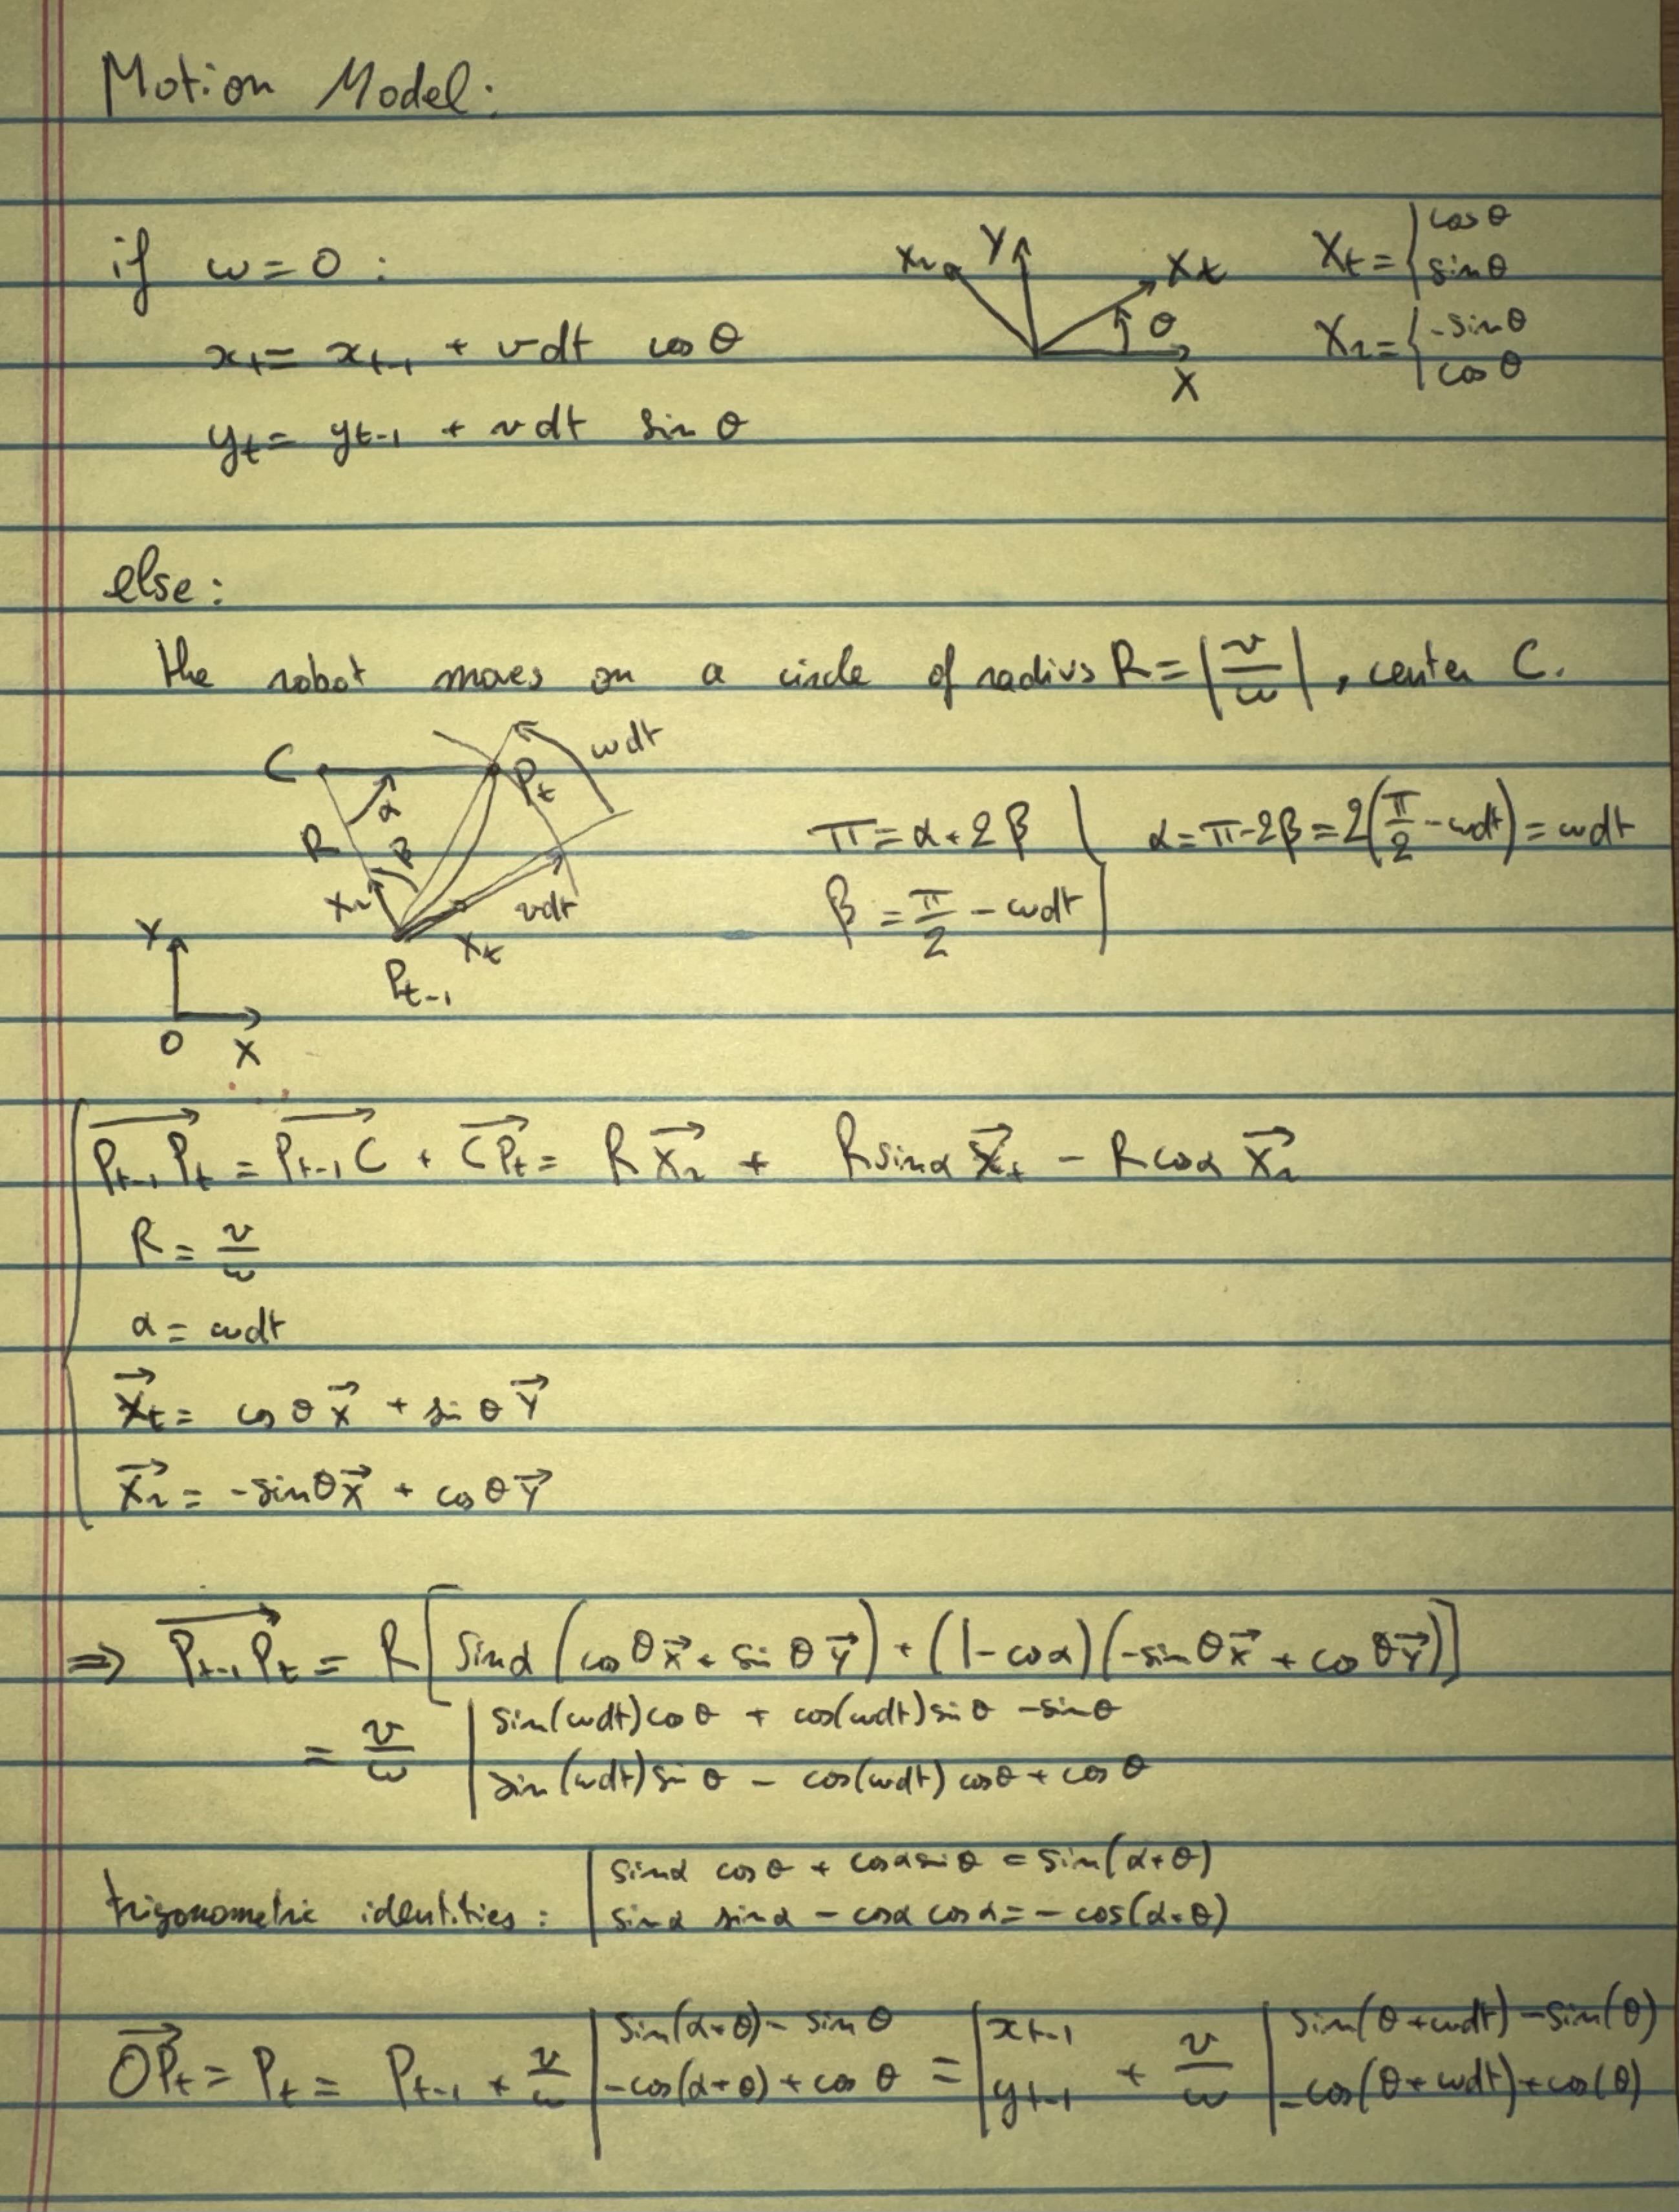
\includegraphics[scale=0.3]{motion_model.jpeg}
\caption{Derivation of the motion model equations}
\label{fig:motmod}
\end{figure}



This motion model is non linear. The terms $1/\omega, \cos(\theta+\omega t), \sin(\theta+\omega t)$ make it non linear. The  special case where $\omega=0$ is linear.

\section{Motion model test on example commands}
The provided sequence of commands has separate translational and rotational speeds. The robot moves in a successions of straight lines (step 1, 3, 5). The initial state is set to $(0,0,0)$.

\begin{figure}
\centering
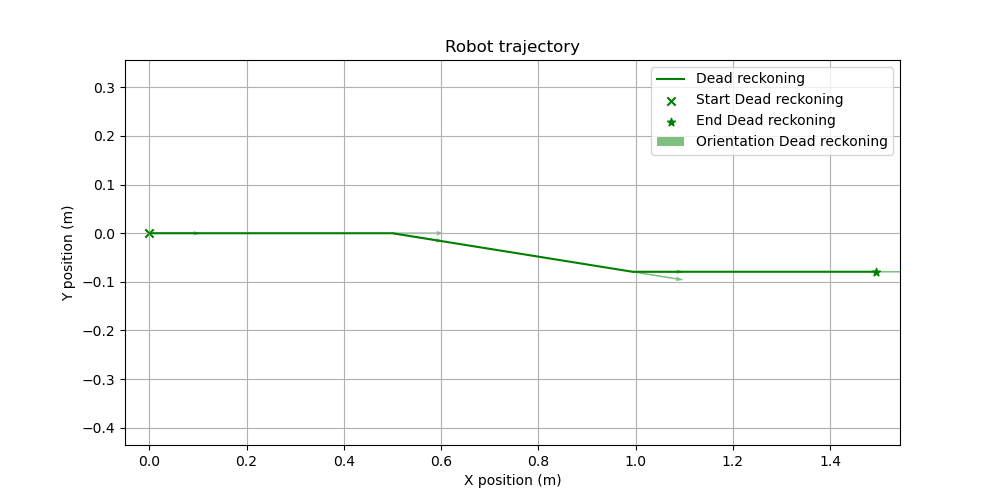
\includegraphics[scale=0.3]{Figure_1.png}
\caption{Robot motion model test on example commands}
\label{fig:figure1}
\end{figure}

\section{Motion model test on robot dataset}
The starting point of the dead-reckoned path uses the ground truth for its initial state. We can observe from \autoref{fig:figure2} that the robot is not following the ground truth. The trajectory loosely tracks until it completely diverges after a few turns, every turn introducing more error. We can observe from \autoref{fig:figure3} that the robot's position error accumulates over time. After $t=150$, the orientation shift is at about $\pi/2$ and we can see that positions start diverging from there. For the remainder of the trajectory we can observe an offset between the orientations, that keeps growing over time.
A number of factors can explain this behavior:
\begin{itemize}
      \item The motion model is simple (does not take into account wheel slip for example).
      \item The geometry of the robot could be slightly different from the assumed one (the wheel base has an impact on a differencial drive robot).
      \item The controls could be noisy.
      \item The power unit and drivetrain can have limitations (power limits, acceleration limits).
      \item We assume the speed to be a step function whereas it should be continuous (no infinite acceleration).

\end{itemize}

\begin{figure}
\centering
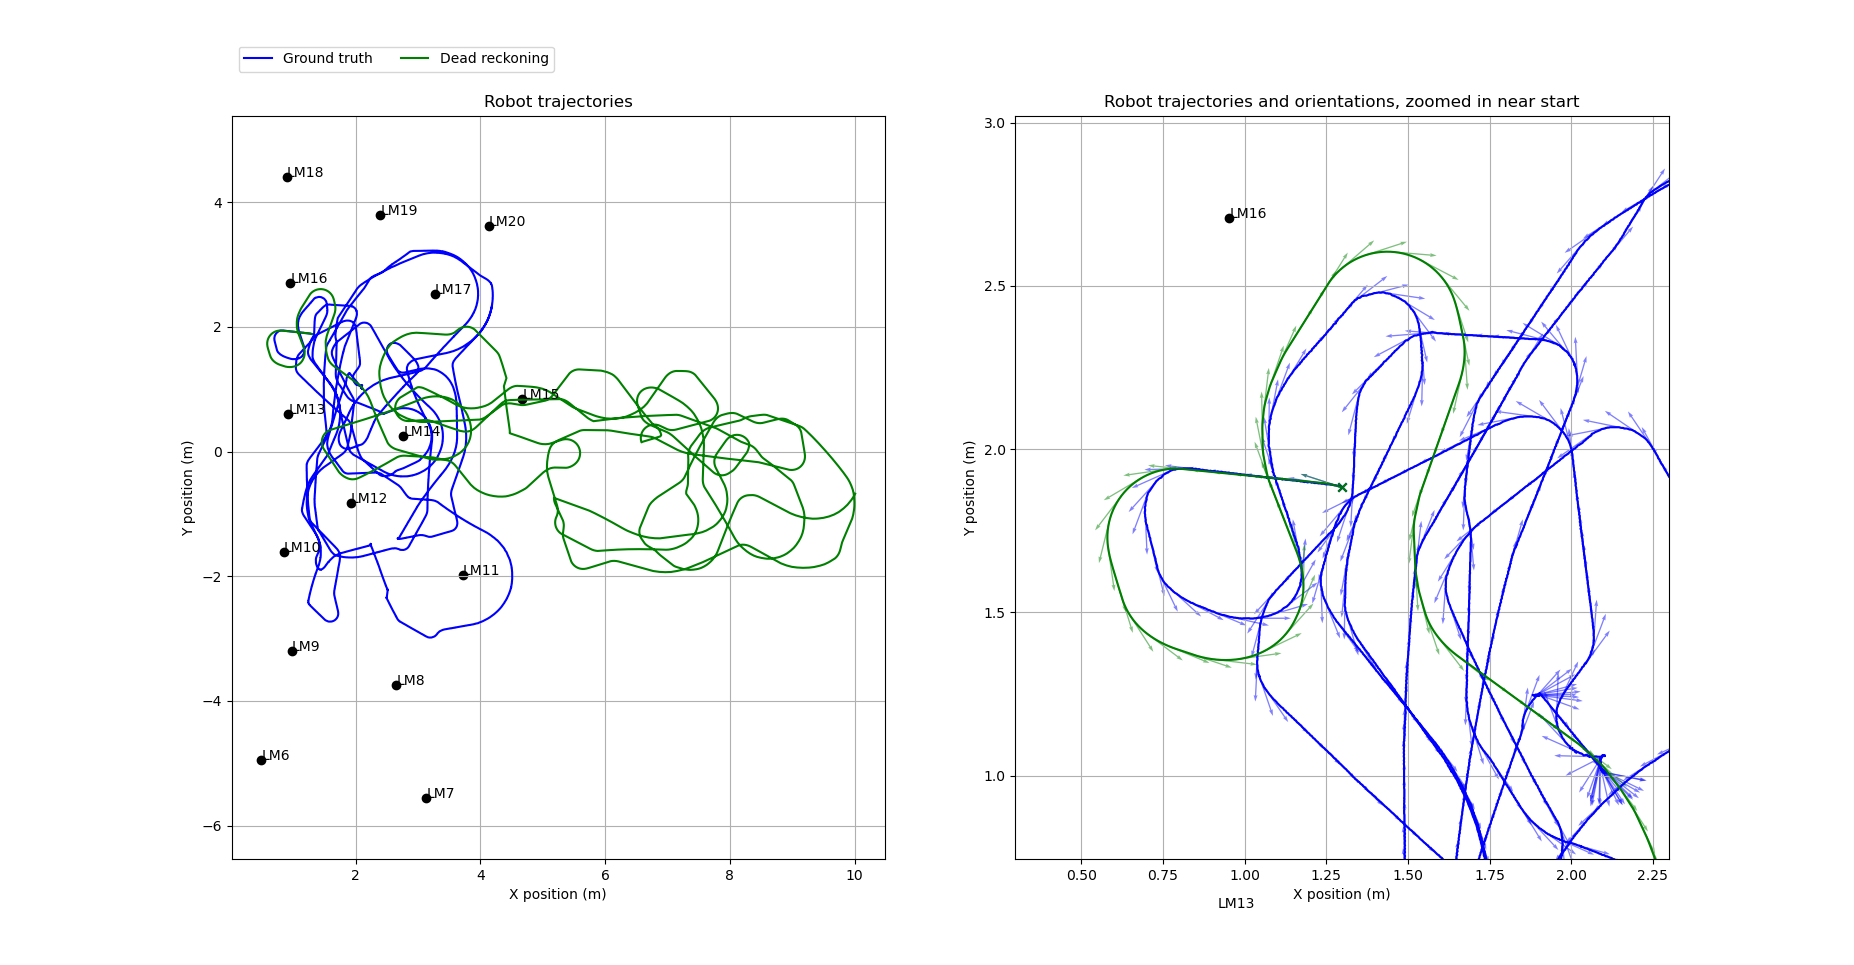
\includegraphics[scale=0.3]{Figure_2.png}
\caption{Robot dead reckoning, compared to ground truth}
\label{fig:figure2}
\end{figure}

\begin{figure}
\centering
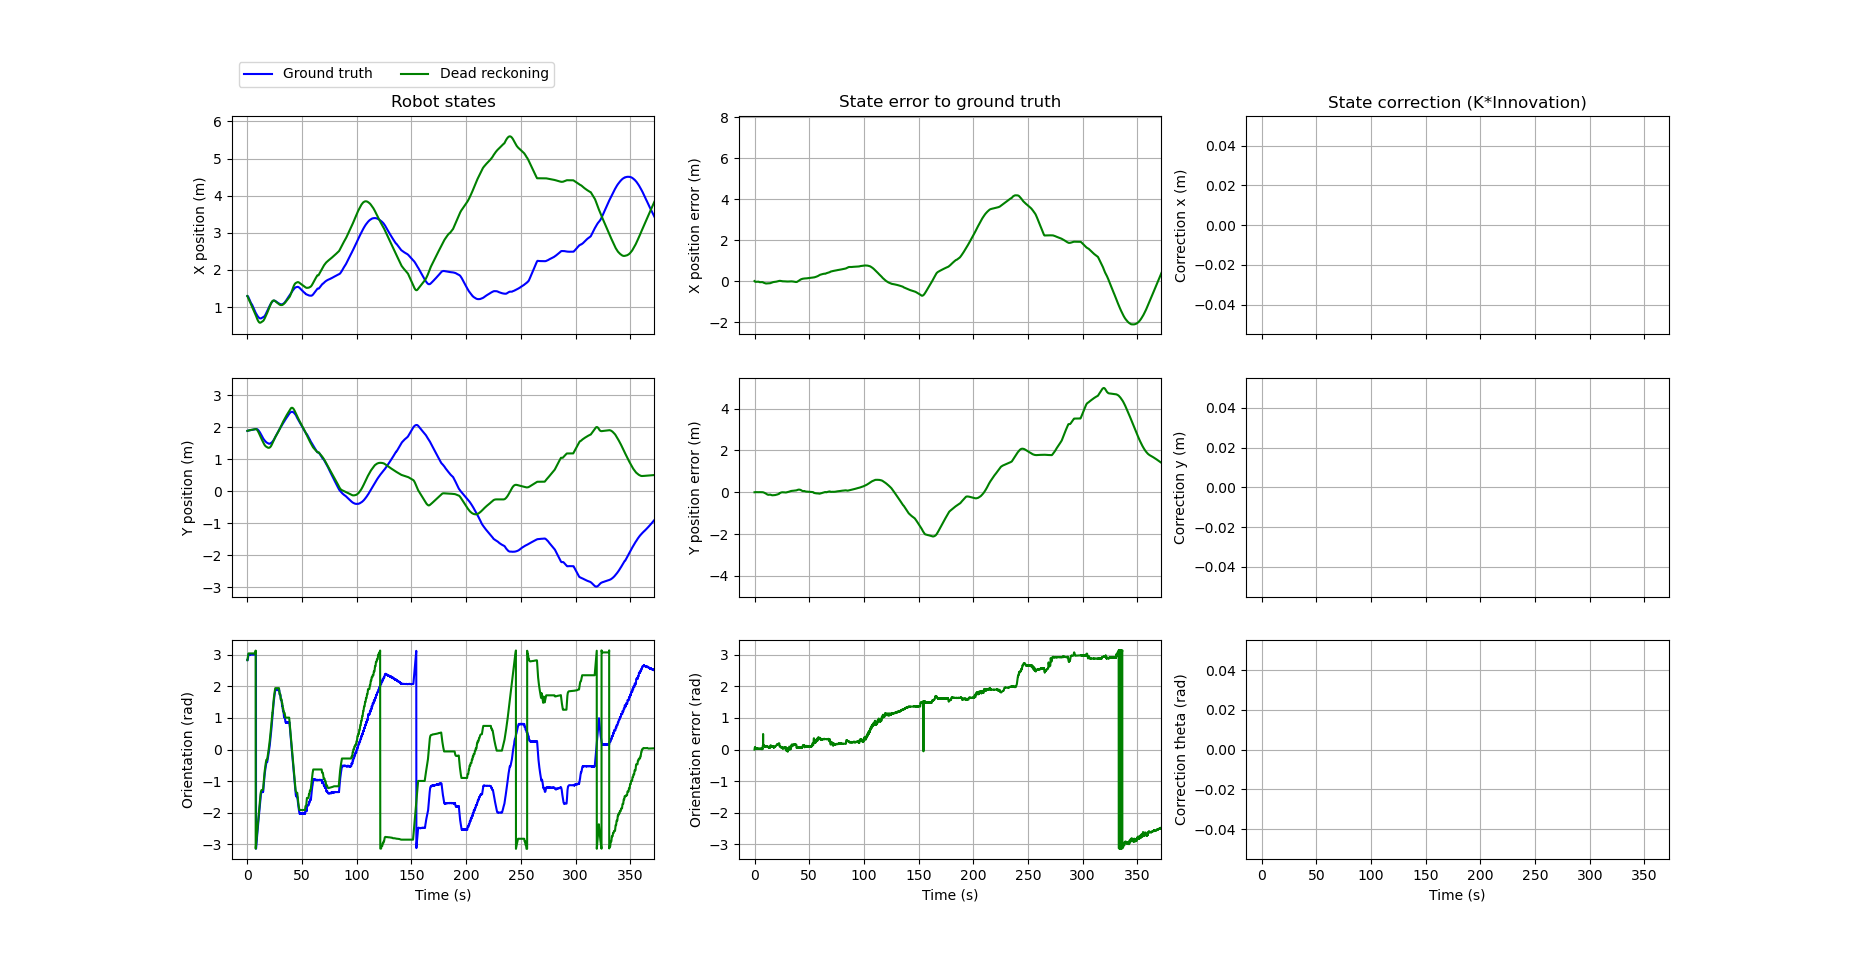
\includegraphics[scale=0.3]{Figure_3.png}
\caption{Robot position and error}
\label{fig:figure3}
\end{figure}

\section{Unscented Kalman Filter}

An unscented Kalman filter (UKF) is in concept similar to a Kalman filter, in that unfolds in two steps. The first step is the prediction: it estimates a posterior belief by means of a motion model based on prior state and a control command applied over a time step. The second step is the correction: it uses a measurement model to create an expected measurement of that posterior belief. This is then compared to the actual measurement, and the posterior belief is adjusted based on the difference between expected and actual measurement. Some knowledge of the uncertainty of both models is required for this correction step (we will discuss further below).

The UKF is different in that it is meant for non-linear models, where the state uncertainty probabilistic parametrisation (gaussian) is not conserved through the model. Instead, the uncertainty is propagated by evaluating sample points (sigma points) through the motion model. A predicted belief mean and covariance is computed from those points. This predicted belief is used to generate new sigma points which are passed through the measurement model. A predicted measurement mean and covariance are constructed.

The sigma points are computed from mean and covariance::
\[\chi(x_{t-1},P_{t-1})=\{\chi_0, \chi_1, \dots, \chi_{7}\}\]
They get propagated through the motion model:
\[Y=f(\chi, u_t)\]
The predicted belief mean and covariance are computed from the propagated sigma points. New sigma points are computed from the predicted belief:
\[Y_{predicted}(\bar{y},P_{yy})=\{y_0, y_1, \dots, y_{7}\}\]
Those get propagated through the measurement model:
\[Z=h(Y_{predicted})\]

The predicted measurement mean and covariance are computed from the propagated measurement sigma points.
From the predicted belief and predicted measurement, the remaining matrix operations are performed to compute the posterior. The Kalman gain is inversely proportional to the measurement noise covariance, so a high covariance means less correction is applied to the posterior (or larger innovations are needed to have an effect).
\[K=P_{yz}P_{zz}^{-1}\]
\[innovation=z_{actual}-z_{predicted}\]
\[posterior=predicted+K*innovation\]
\[P_{posterior}=P_{predicted}-K*P_{zz}*K^T\]

Sources: 

\href{https://ahrs.readthedocs.io/en/latest/filters/ukf.html}{Unscented Kalman Filter - AHRS Documentation}

\href{https://groups.seas.harvard.edu/courses/cs281/papers/unscented.pdf}{The Unscented Kalman Filter for Nonlinear Estimation - Wan and Merwe}

\section{Measurement model}

The measurement model takes the predicted belief $(x, y, \theta)$ as inputs, as well as knowledge about the space, in this case the measured (assumed true) positions of the landmarks (those are available via the Landmark Groundtruth file).
The model outputs an estimated measurement range and bearing.

The derivation of the measurement model is shown in \autoref{fig:measmod}. The range is the euclidean distance between the robot and the landmark. The bearing is the angle between the robot's orientation and the line connecting the robot and the landmark.

\begin{figure}
\centering
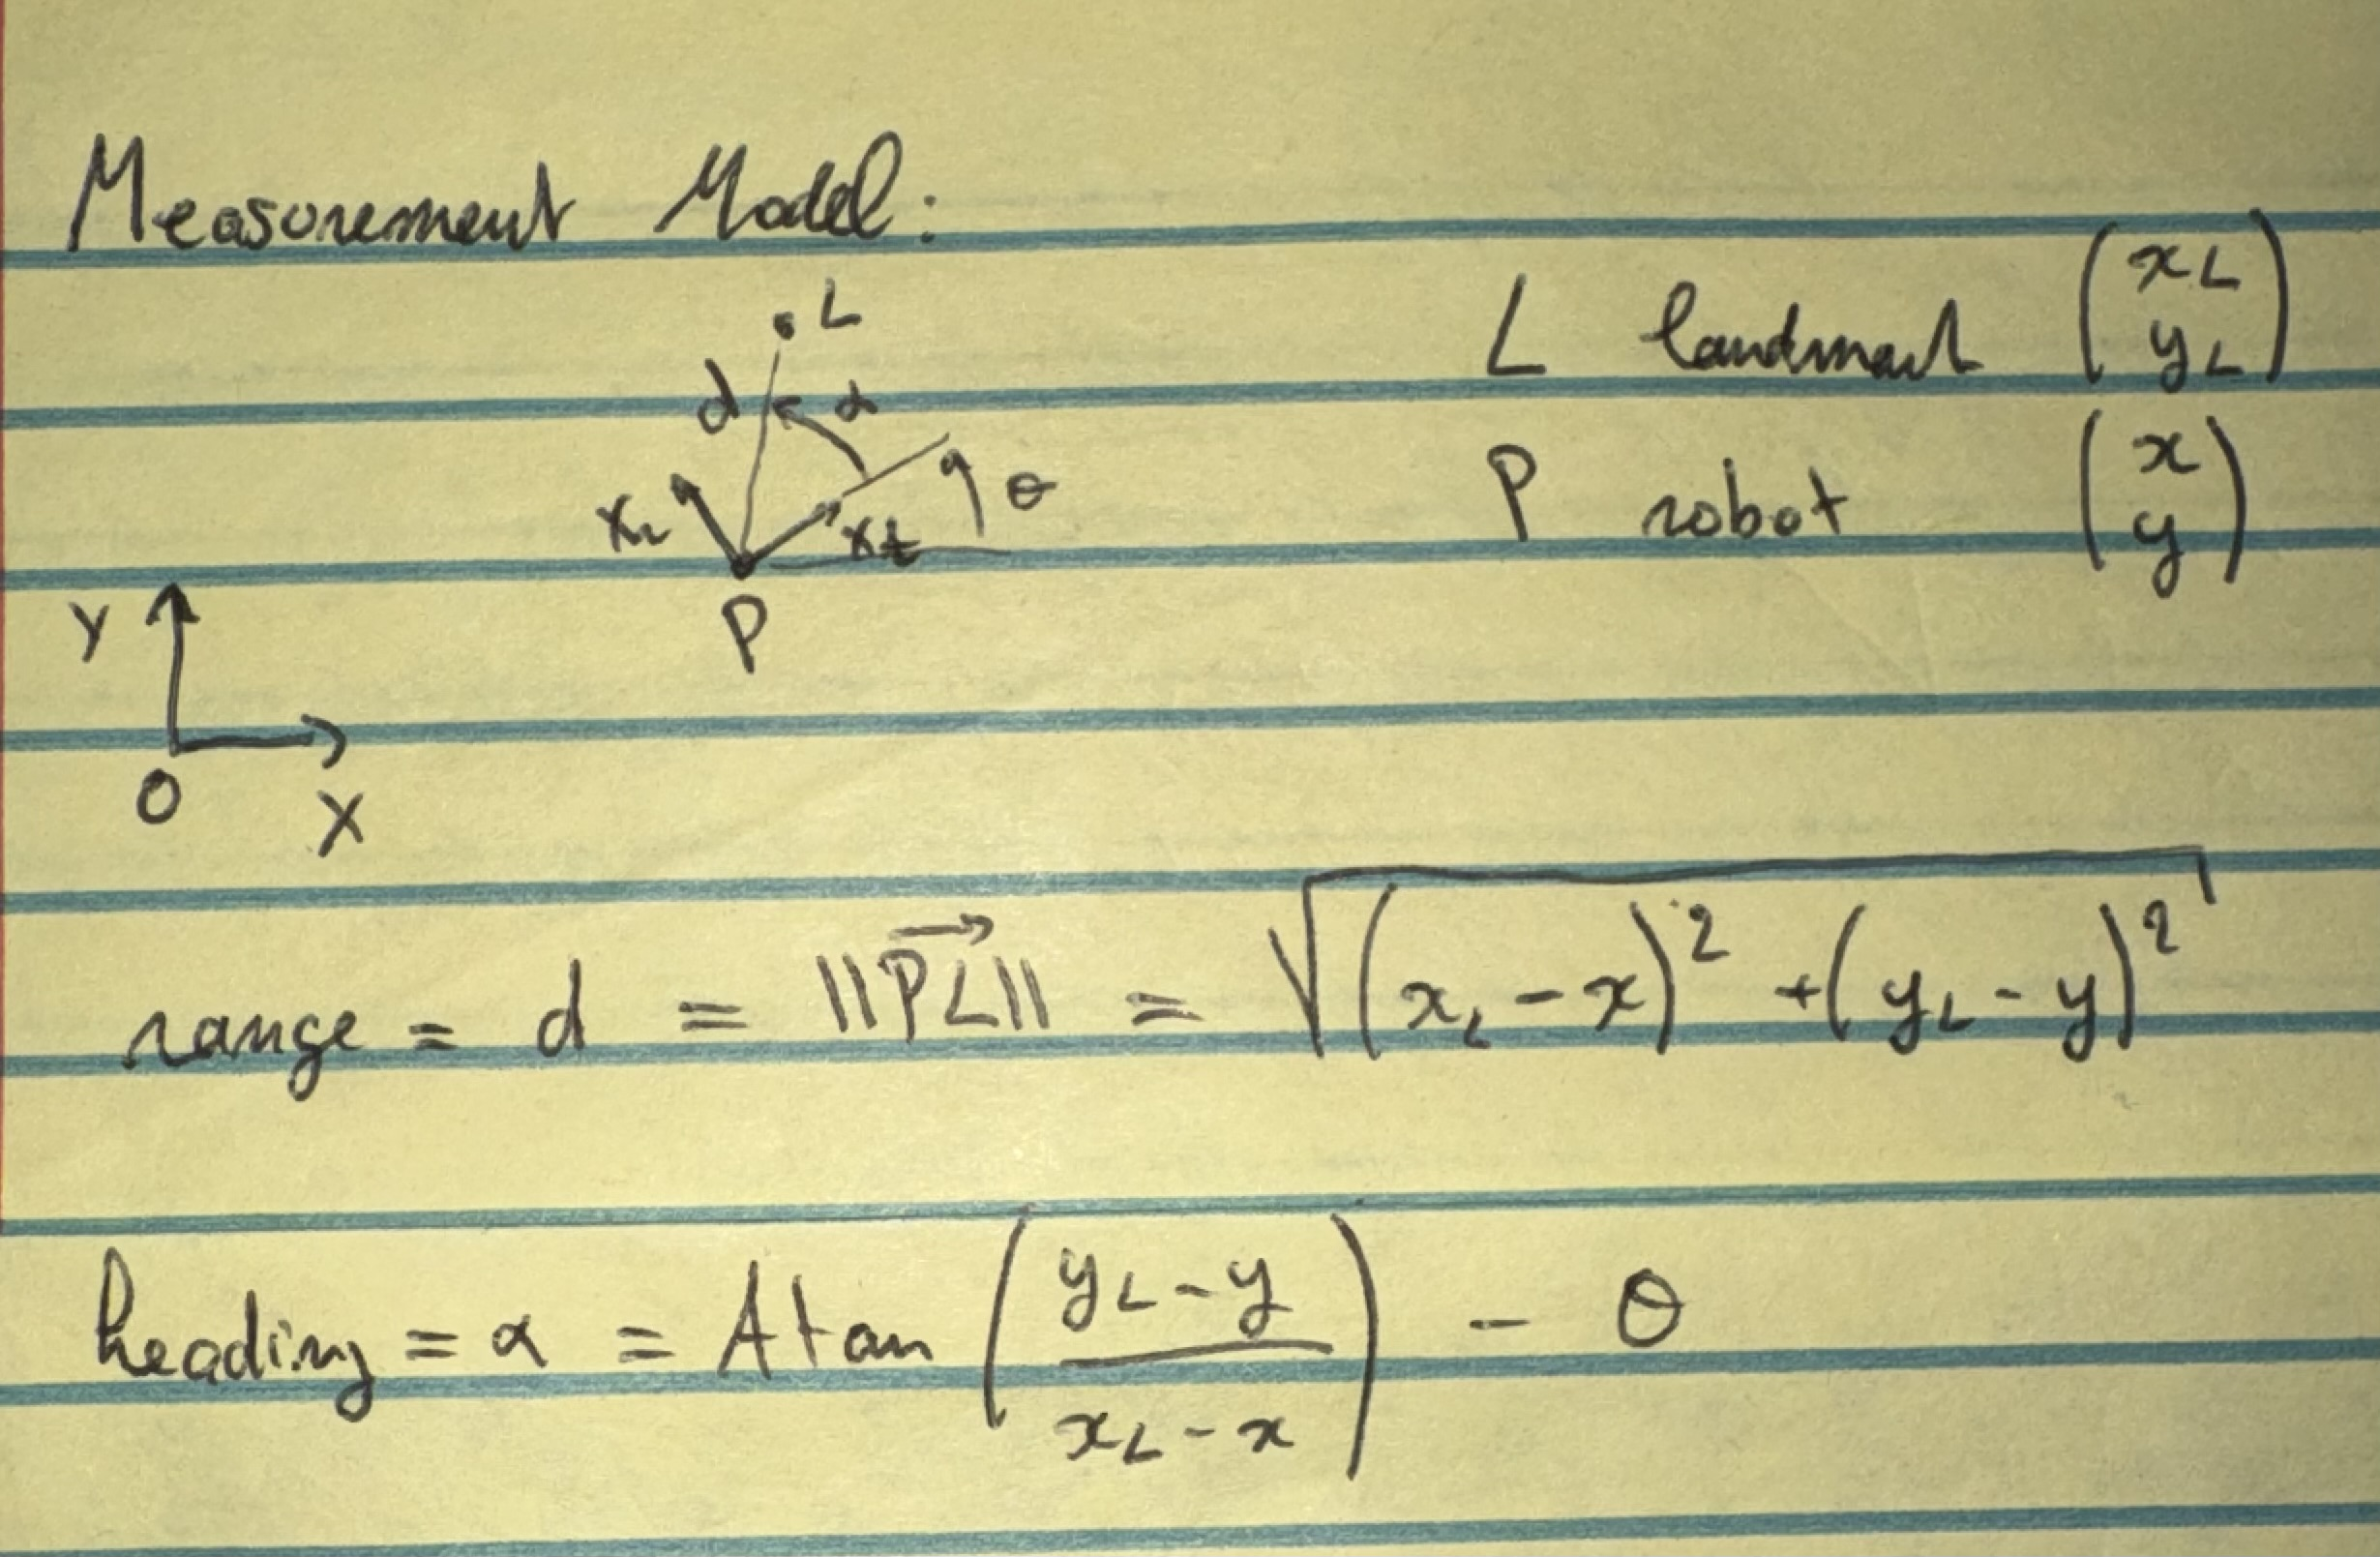
\includegraphics[scale=0.3]{measurement_model.jpeg}
\caption{Robot position and error}
\label{fig:measmod}
\end{figure}

The measurement data reads landmark barcodes. Those need to be converted to the subject number between 6 and 20 so that they can be paired with the ground truth landmark data. This is done using the barcodes file.



\section{Test of measurement model on robot data}
The measurement model does not add noise and the positions provided are assumed to be the known robot position. The measurement model successfully finds all landmarks with zero error.

\vspace{1cm}
\large{Part B}
\normalsize{}

\section{Filter implementation}

In order for the filter to be implemented on this dataset, some attention needs to be paid to synchronize the data. The controls and the measurements are on different time grids. We interpolate the controls data over a fixed timestep chosen to be 0.05s. This timestep can be updated but seems to have little effects on the overall behavior. The measurements are grouped to the nearest timestep. Because of the lower accuracy of those measurement, this will prove acceptable.

Special attention also needs to be paid when working with angles. Anytime an angle is manipulated, we will normalize it between $]-\pi,\pi]$. We will use the circular mean for means calculations (source: \href{https://en.wikipedia.org/wiki/Circular_mean}{Wikipedia: Circular mean}).


\section{Comparison to dead reckoning}
Let us look at the data and try to undestand the order of magnitude of the covariance matrices.
Looking at the control data set (resampled at 0.05s intervals), the we find $\nu<0.1m/s$ and $\omega<0.6rad/s$. This means the upper bound a state will evolve after a timestep is $0.005m$ and $0.03rad$. We expect the motion model to be reasonably accurate, we will make an assumption that it is at least 80\% accurate. This means our process noise covariance matrix will have for diagonal elements $\sigma_x^2=\sigma_y^2=(0.005/5)^2=10^{-6},\sigma_\theta^2=(0.03/5)^2=3.6\e{-5}$). We have no data on the measurements accuracy or the robot sensor. It is likely that the measurements are noisy, orders of magnitude higher than the process noise covariance. We will explore this further below when tuning the parameters. For now, we will assume a starting point of $\sigma_{range}^2=0.1^2=10^{-2}, \sigma_{bearing}^2=(6*3.14/180)^2=10^{-2}$.


Now looking at the robot dataset, we can find that the first measurement is collected at $t=11.100s$. Until then, the filter is not providing any correction and the trajectory matches the dead-reckoned path.
However, once the first measurement is collected, the filter starts correcting the trajectory. We can observe from figure 4 that the UKF trajectory mostly tracks the ground truth.

\begin{figure}
\centering
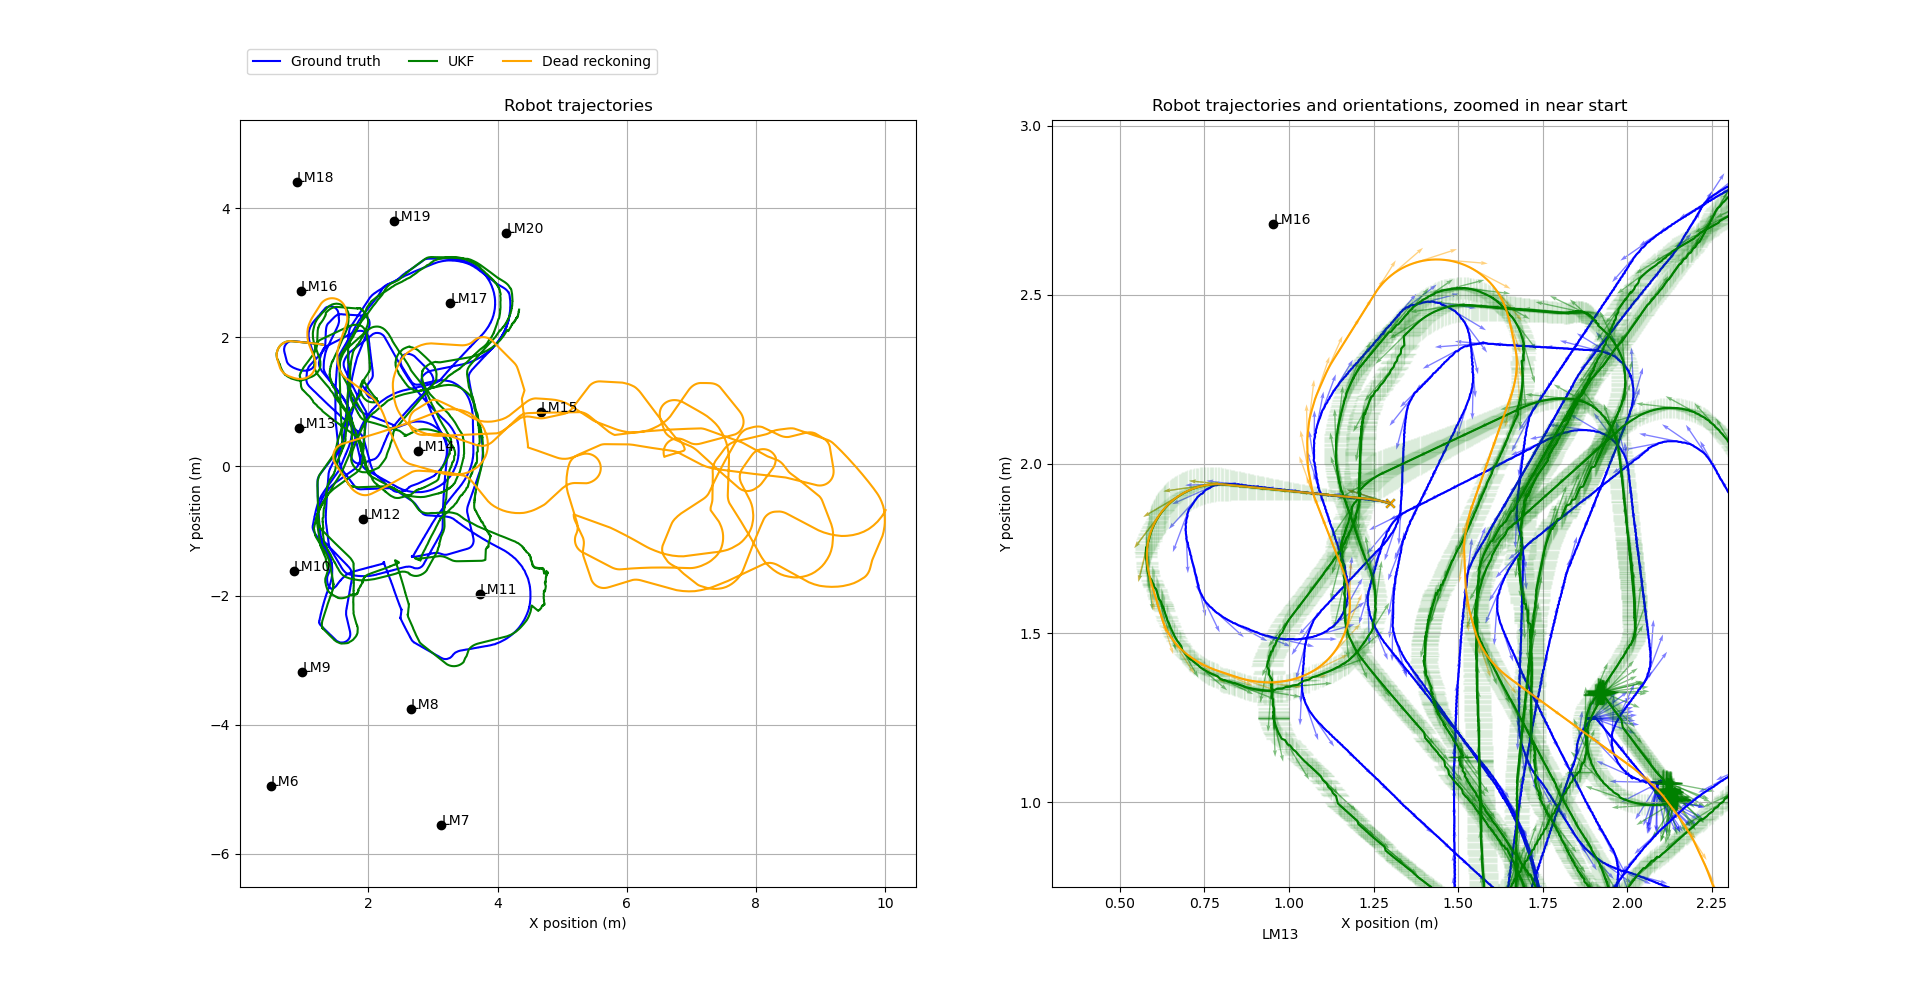
\includegraphics[scale=0.3]{Figure_4.png}
\caption{Robot trajectory predictions with and without UKF. The figure on the right shows the 95 percent confidence interval on position for the UKF trajectory.}
\end{figure}


\begin{figure}
\centering
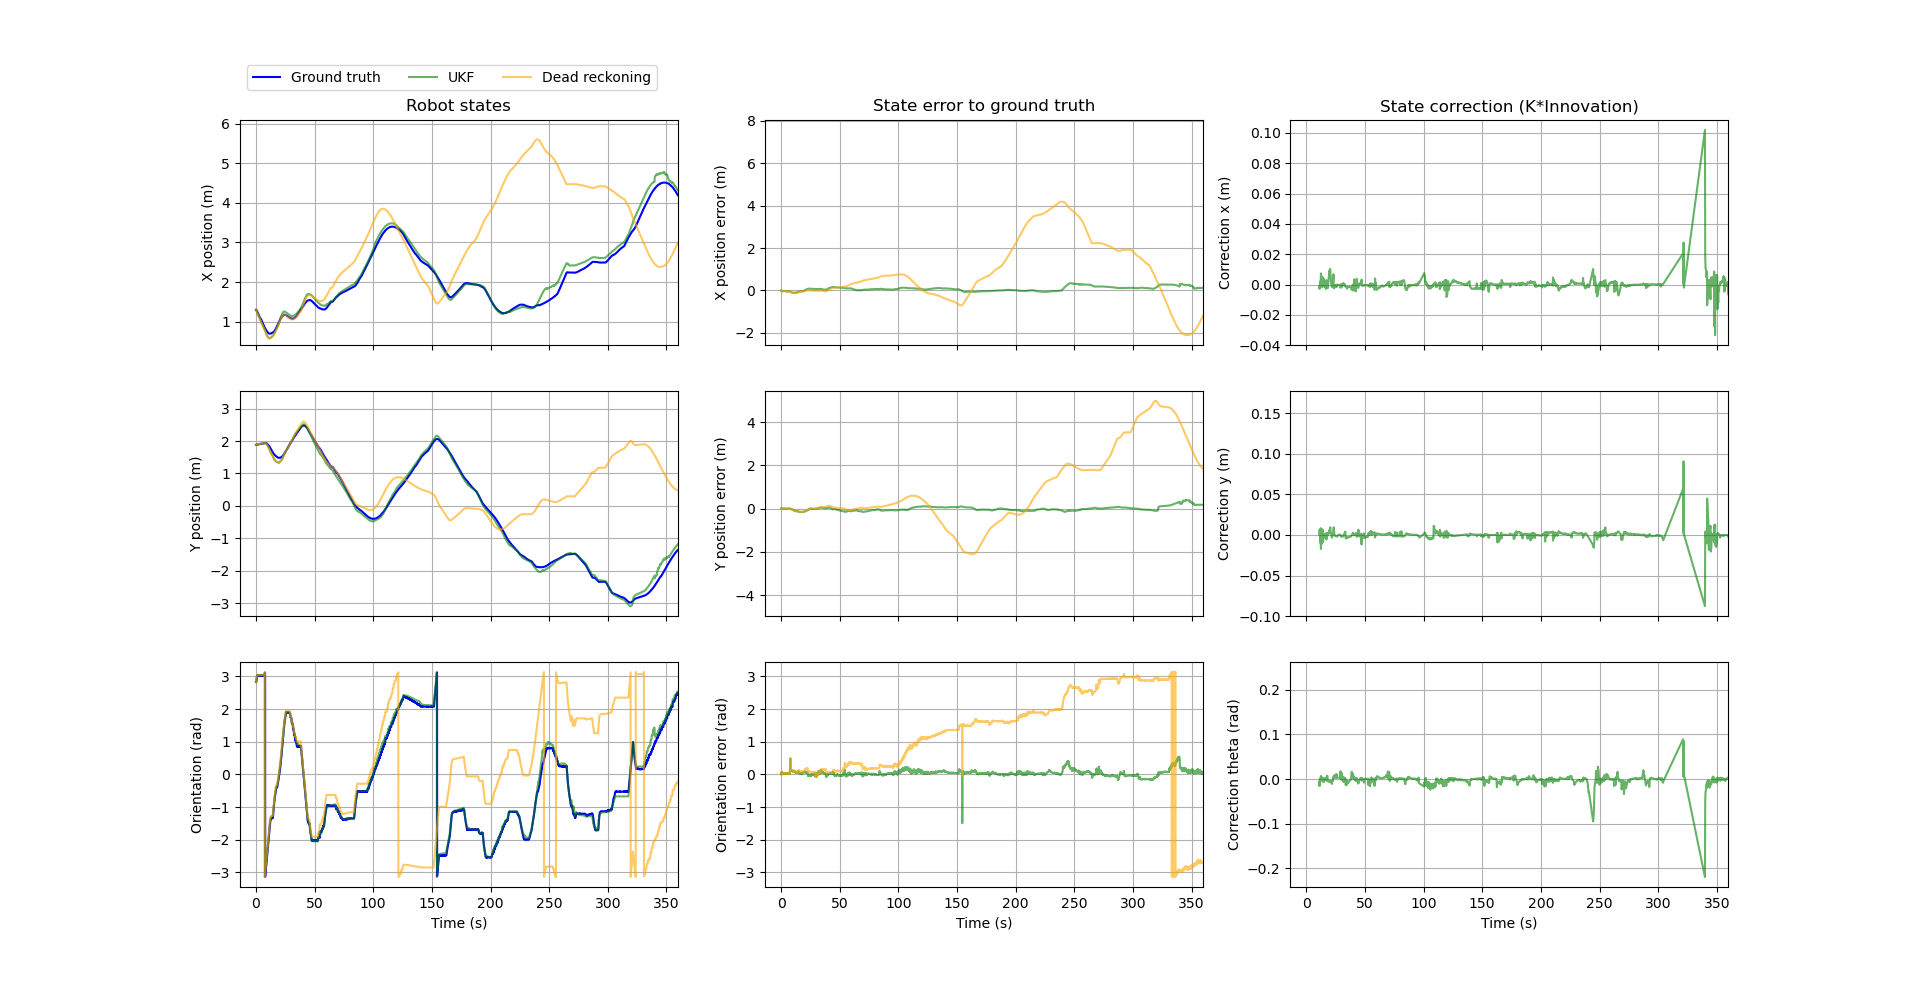
\includegraphics[width=\textwidth]{Figure_5.png}
\caption{Robot states and errors (UKF vs dead reckoning)}
\end{figure}

\section{Filter analysis}
We will in this section perform an exploration of the different filter parameters. We need to be paying attention to the following parameters:
\begin{itemize}
      \item Initial state and its covariance
      \item Process noise covariance
      \item Measurement noise covariance
      \item Alpha
\end{itemize}

We have limited data available on the robot and its controls and sensors, the different covariance matrices (initial state covariance, process noise covariance and measurement noise covariance) have been assumed as diagonal matrices. All the variables in each matrix are considered to be statistically independent of one another.


\subsection{Process and measurement noise covariance}
With the process noise covariance matrix set to what is believed to be a reasonable value based on the motion model, we can start our exploration on the measurement noise covariance. There is limited knowledge on the sensors being used on the robot.
An estimation of the measurement noise covariance can be estalish iteratively. We will try multiples (1, 0.01, 100) of our earlier guess $\sigma_{range}^2=10^{-2}, \sigma_{bearing}^2=10^{-2}$. The plot in \autoref{fig:figure6} shows the trajectory predictions for different noise parameters. The plots in \autoref{fig:figure7} and \autoref{fig:figure8} show the states, errors, predicted measurements and innovations for the different noise parameters. The 95\% confidence interval is shown (defined as +/-2*stddev), to get an idea of the uncertainty of the predictions.

We find, as reported in \autoref{fig:figure7} and \autoref{fig:figure8}, that the measurement noise covariance has a strong impact on the behavior of the filter. The Kalman gain, which controls how much the posterior is corrected based on the innovation (difference between expected and actual measurement) is directly linked to the ratio between process noise covariance and measurement noise covariance. A higher measurement noise covariance means more uncertainty, and less confidence in the measurements. The Kalman gain will be lower, we will need a large innovation (error) to correct the state (and vice versa, a low measurement noise covariance means we can correct the state with a smaller innovation).

A low measurement noise covariance matrix leads to high overcorrection and very noisy posterior predictions. If the noise covariance is too low, the state is updated with an equivalent control*dt that shows displacement beyond what can be expected feasible.

A high measurement noise covariance matrix leads to oversmoothing of the trajectory, the correction step provides minimal adjustments which leads to delayed corrections (the error needs to be large for the correction to take effect). For very large (order of magnitude larger of 5 or more then the process noise covariance), the model will ignore the measurements and the robot be left dead reckoning.

It seems that a difference in order of magnitude of 4 leads to our best results, which is actually consistent with the initial guess. This leads to the smoothest (not over-corrected) and most accurate trajectory. Additionally, one can observe that shifting both process and measurement noise covariance higher or lower in pairs has little impact on the trajectory.

\begin{figure}
\centering
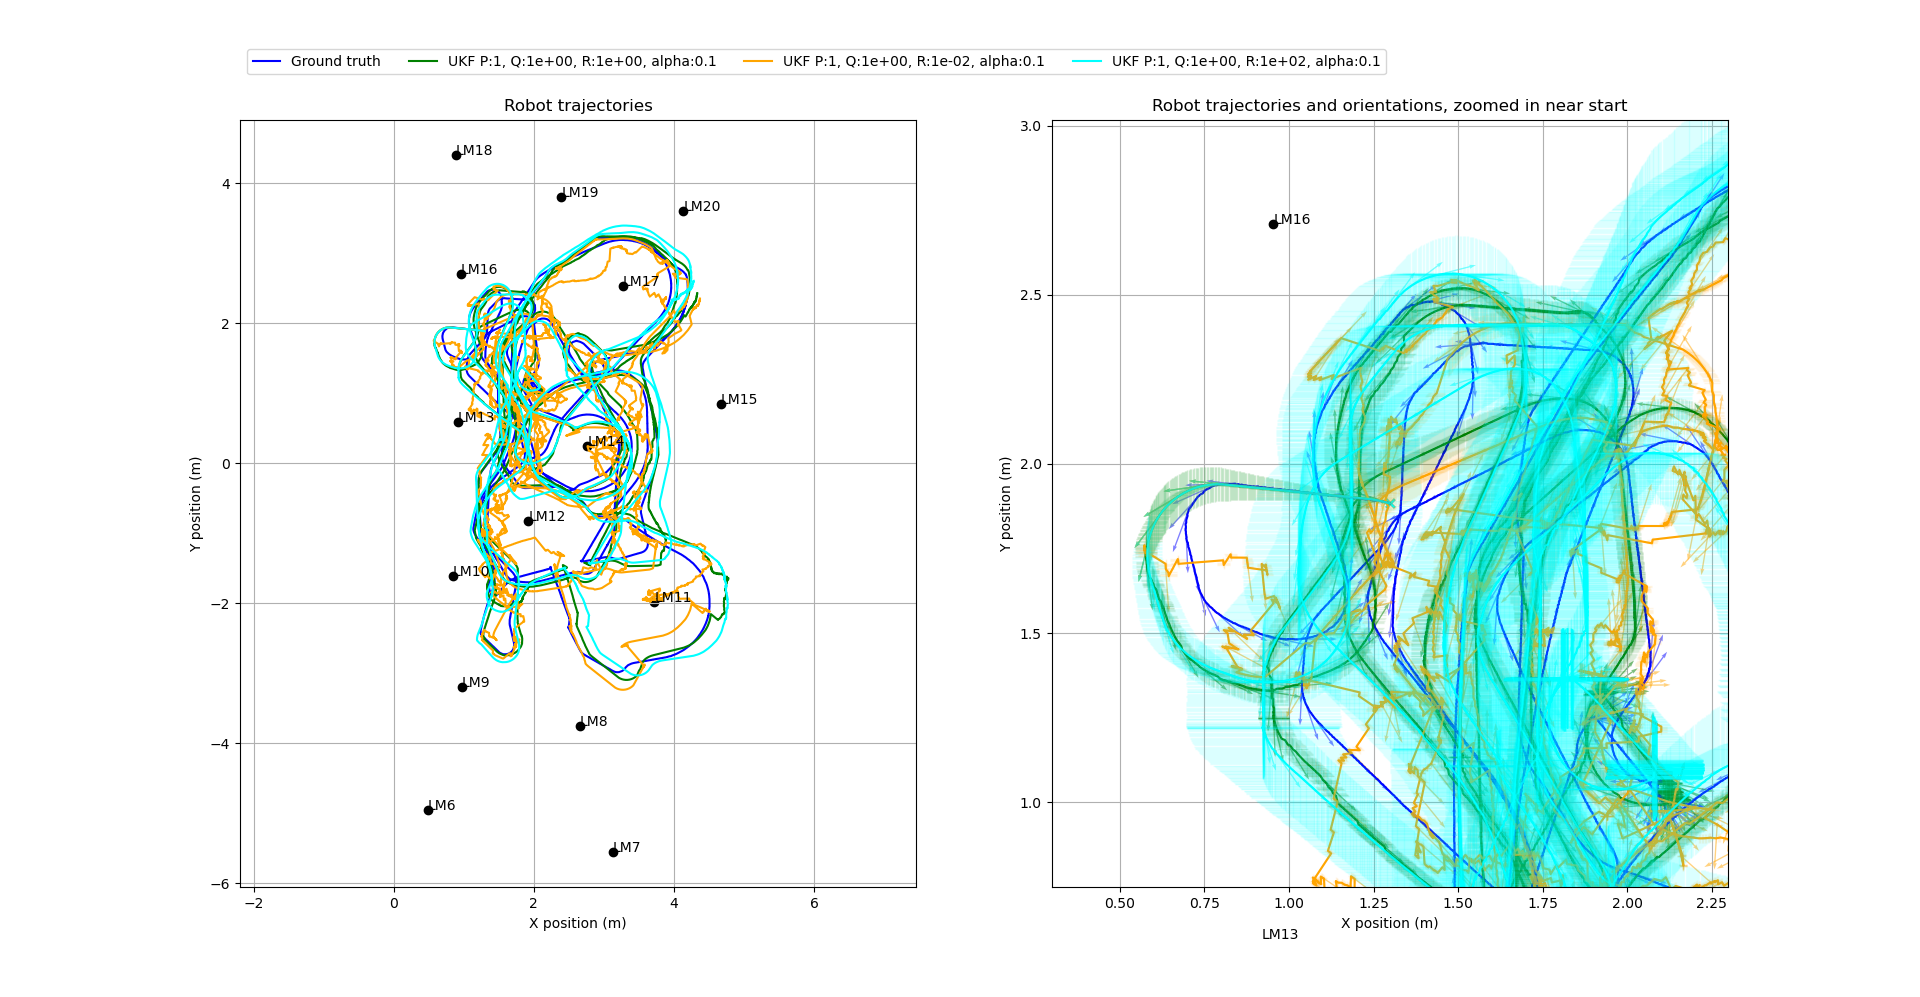
\includegraphics[width=\textwidth]{Figure_6.png}
\caption{Robot trajectory predictions for different UKF noise parameters. The 95 percent confidence interval on position is shown on the right figure. Green is our baseline UKF, Orange and Cyan used a measurement noise covariance 100 times lower and higher respectively.}
\label{fig:figure6}
\end{figure}


\begin{figure}
\centering
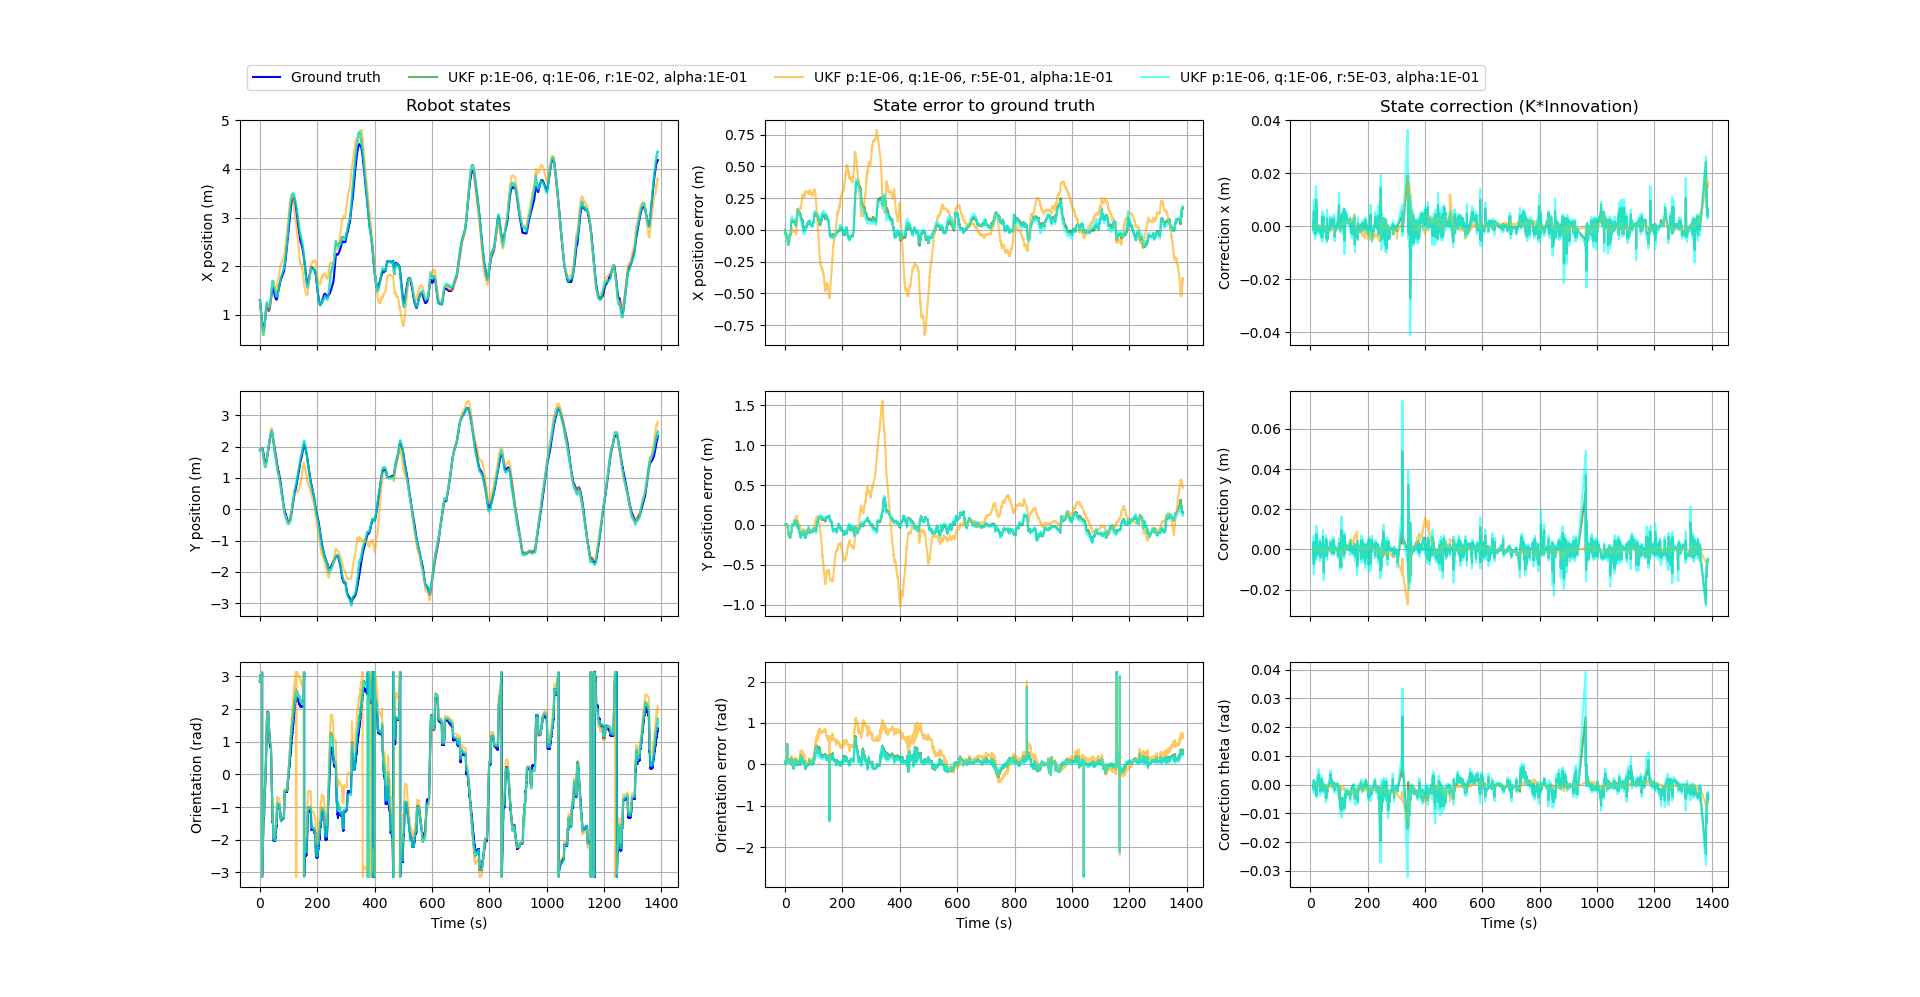
\includegraphics[width=\textwidth]{Figure_7.png}
\caption{Robot states and errors for different UKF noise parameters}
\label{fig:figure7}
\end{figure}

\begin{figure}
\centering
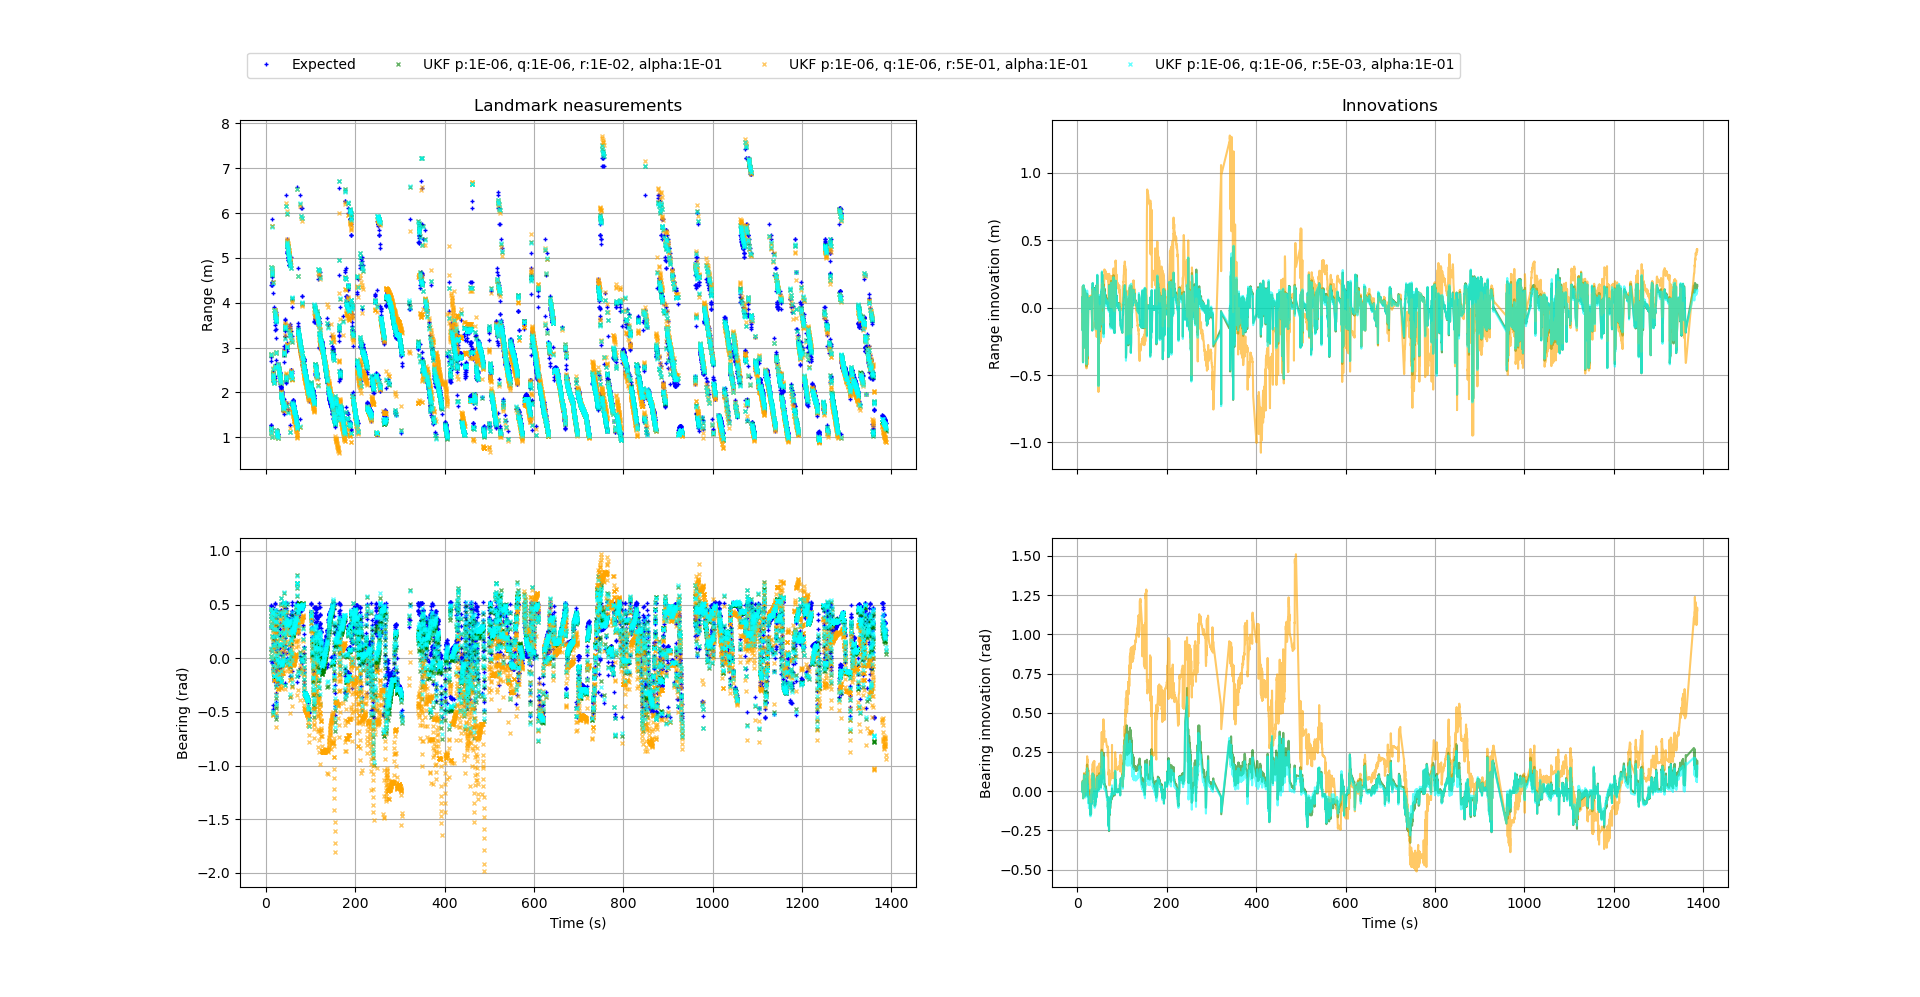
\includegraphics[width=\textwidth]{Figure_8.png}
\caption{Robot predicted measurements and innovations for different UKF noise parameters}
\label{fig:figure8}
\end{figure}

\subsection{Initial state and its covariance}
Adding noise to the starting point and/or increasing the initial state covariance seems to have limited impact. For a known starting point, the initial state covariance has little impact. Once the first measurements are available, the filter quickly converges back near the true state and all estimations agree with one another.

\subsection{Alpha}
Alpha controls the spread to the mean when creating the sigma points. After iteratiing for $\alpha=[0.01, 0.1, 1]$, it does not seem to have much of an impact on the behavior of the filter. This gives confidence in the capacity of the sigma points in capturing the non-linear behavior and the assumption about the state estimation as a gaussian (we have a single target / we do not expect a multi modal distribution).

\subsection{No measurement}
If no measurement is available, the filter will only perform the prediction step. The posterior will be equal to the predicted belief. The uncertainty on the state will increase as the process noise covariance is added to the covariance of the predicted belief (as can be observed in \autoref{fig:figure6} from $t=0$ until sometime after the first turn when the first measurement occurs).

\subsection{Multiple measurements}
If several measurements are found for a given time step, the correction step loops over the measurements one by one, using the corrected posterior as the new input for the next measurement.

\subsection{Final considerations}

The initial guess on the process and measurement noise covariance leads to the best results found. 
The average distance error is 0.107m and the average bearing error is 0.049rad (2.8 degrees).


\end{document}
